% ====================================================================================
\chapter{从有限维到无限维：变分法}
% ====================================================================================

\section*{引言：兄弟之争与一个反直觉的问题}

1696年6月，数学杂志《学术纪事》（Acta Eruditorum）上出现了一则挑战公告。瑞士数学家 Johann Bernoulli 向全欧洲数学家发出挑战：
\storynote{Bernoulli家族}{数学史上最传奇的家族！三代人出了八位杰出数学家。Johann和哥哥Jakob经常公开争吵、互相攻击，却都做出了一流贡献。Johann甚至试图把儿子Daniel的工作据为己有。家族内斗之激烈，堪比宫斗剧。}

\begin{quote}
\textit{给定两点 A 和 B，A 不在 B 的正上方。求一条连接它们的曲线，使得一个小球仅在重力作用下，从 A 滑到 B 所需时间最短。}
\end{quote}

这就是著名的\textbf{最速降线问题}（Brachistochrone，来自希腊语"最短"和"时间"）。

\subsection*{直觉的失败}

乍一看，答案似乎显而易见——直线不就是两点之间最短的路径吗？但 Johann 狡黠地补充道："虽然直线路程最短，但它不是时间最快的路径。"

让我们用一个简单的计算来理解为什么。

\begin{example}[直线 vs 折线]
假设 A 在原点，B 在 $(4, -3)$（向右 4 米，向下 3 米）。小球从静止开始下滑。

\textbf{方案1：走直线}
\begin{itemize}
    \item 路径长度：$\sqrt{4^2 + 3^2} = 5$ 米
    \item 平均加速度：重力在斜面方向的分量 $g \sin\theta = g \cdot \frac{3}{5} = 0.6g$
    \item 用 $s = \frac{1}{2}at^2$ 估算：$t_1 \approx \sqrt{\frac{2 \times 5}{0.6g}} \approx 1.31$ 秒
\end{itemize}

\textbf{方案2：先陡后缓}（先垂直下降 2 米，再沿斜面到 B）
\begin{itemize}
    \item 第一段：垂直下降 2 米，加速度是完整的 $g$
    \item 到达第一段底部时，速度 $v = \sqrt{2g \times 2} = \sqrt{4g} \approx 6.3$ m/s
    \item 第二段：已经有了初速度，虽然路程长了，但跑得快！
    \item 粗略估算：$t_2 \approx 1.15$ 秒
\end{itemize}

\textbf{结论}：绕远路反而更快！
\end{example}

\begin{figure}[htbp]
\centering
\begin{tikzpicture}[scale=0.9]
    % 坐标轴
    \draw[->] (-0.5,0) -- (6,0) node[right] {$x$};
    \draw[->] (0,0.5) -- (0,-4.5) node[below] {$y$（向下为正）};
    
    % 起点和终点
    \fill[red] (0,0) circle (3pt) node[above left] {A};
    \fill[red] (4,-3) circle (3pt) node[right] {B};
    
    % 直线路径
    \draw[blue, thick, dashed] (0,0) -- (4,-3);
    \node[blue] at (2.5,-0.8) {直线：路程短};
    \node[blue] at (2.5,-1.3) {\small 但起步慢};
    
    % 摆线路径（近似）
    \draw[red, very thick] (0,0) .. controls (0.3,-1.5) and (0.8,-2.5) .. (2,-3.2) 
                           .. controls (3.2,-3.5) and (3.8,-3.2) .. (4,-3);
    \node[red] at (1,-3.5) {摆线：路程长};
    \node[red] at (1,-4) {\small 但先加速后匀速};
    
    % 小球示意
    \shade[ball color=gray] (0.5,-0.3) circle (0.15);
    \draw[->, thick] (0.5,-0.3) -- (0.5,-0.8) node[right] {\small $g$};
\end{tikzpicture}
\caption{最速降线问题：直线不是最快路径}
\end{figure}

\sidenoteplain{这就像开车去机场：高速公路虽然绑了一圈，但因为速度快，总时间可能比走市区直线更短。}

\begin{tcolorbox}[colback=green!5, colframe=green!60!black, title=学完这章，你将能够...]
\begin{itemize}
    \item 写出给定泛函的Euler-Lagrange方程
    \item 求解最速降线、测地线、最小曲面等经典变分问题
    \item 把"连续曲线优化"离散化为"有限维向量优化"
    \item 处理带端点约束、等周约束的变分问题
    \item 理解变分法与有限元方法的深刻联系
\end{itemize}
\end{tcolorbox}

\subsection*{历史插曲}

这个挑战引发了一场数学竞赛。参与者包括当时最顶尖的数学家：Leibniz、L'Hôpital、以及 Johann 的哥哥 Jakob Bernoulli。

最戏剧性的一幕发生在英国。问题被转交给了已经退休的 Isaac Newton。据说牛顿收到问题时已是下午四点，但他整个晚上都在工作，到凌晨四点就解决了。

牛顿选择匿名发表解答。但当 Johann 看到那个优雅的证明时，他立刻认出了作者："我从爪子认出了狮子（Tanquam ex ungue leonem）。"
\storynote{Isaac Newton}{牛顿当时53岁，已从剑桥退休，正担任皇家铸币厂厂长。据说他对这个"挑衅"非常恼火，一晚上就解决了问题。有人问他为何匿名发表，他说："我不喜欢被外国人用数学题来戏弄。"}

\textbf{答案}：最速降线是一条\textbf{摆线}（cycloid）——圆在直线上滚动时，圆周上一点的轨迹。

\begin{figure}[htbp]
\centering
\begin{tikzpicture}[scale=0.8]
    % 地面
    \draw[thick] (0,0) -- (8,0);
    
    % 滚动的圆（多个位置）
    \foreach \x in {0.8, 2.4, 4.0, 5.6} {
        \draw[gray] (\x, 0.8) circle (0.8);
    }
    
    % 摆线轨迹
    \draw[red, very thick, domain=0:2*pi, samples=100] 
        plot ({0.8*(\x - sin(\x r))}, {0.8*(1 - cos(\x r))});
    
    % 标记点
    \fill[red] (0,0) circle (3pt);
    \fill[red] ({0.8*(2*pi)}, 0) circle (3pt);
    
    % 标注
    \node at (4, -0.8) {圆滚动时，圆周上一点画出摆线};
\end{tikzpicture}
\caption{摆线的生成：圆在直线上滚动}
\end{figure}

\begin{insightbox}
最速降线问题揭示了一个深刻的原理：\textbf{最优不等于最短}。

在有约束的系统中，"走捷径"往往不是最好的策略。这个思想贯穿整个优化理论。
\end{insightbox}

% ------------------------------------------------------------------------------------
\section{核心问题：优化的对象是什么？}

\subsection{从"找最优数"到"找最优曲线"}

让我们先回顾一下不同类型的优化问题：

\begin{center}
\renewcommand{\arraystretch}{1.5}
\begin{tabular}{c|c|c|c}
\toprule
\textbf{问题类型} & \textbf{优化对象} & \textbf{目标} & \textbf{例子} \\
\midrule
单变量优化 & 一个数 $x$ & $\min f(x)$ & 找利润最大的价格 \\
\midrule
多变量优化 & 向量 $\mathbf{x} = (x_1, \ldots, x_n)$ & $\min f(\mathbf{x})$ & 找最优的生产计划 \\
\midrule
\textbf{变分问题} & \textbf{函数} $y(x)$ & $\min J[y]$ & 找最快的下滑曲线 \\
\bottomrule
\end{tabular}
\end{center}

变分问题的特殊之处在于：我们要找的不是一个数，也不是几个数，而是\textbf{整条曲线}。

\subsection{泛函：以函数为输入的函数}

普通函数把数变成数：$f: \mathbb{R} \to \mathbb{R}$，比如 $f(x) = x^2$。

\textbf{泛函}（functional）把函数变成数：$J: \{\text{函数}\} \to \mathbb{R}$。
\clarify{泛函的"泛"字表示"广泛"——它比普通函数更一般。普通函数吃数字吐数字，泛函吃函数吐数字。你可以把泛函想象成一个"评分系统"：给它一条曲线，它告诉你这条曲线"有多好"。}

\begin{definition}[泛函]
泛函是"以函数为输入，以数字为输出"的映射。给定一条曲线 $y(x)$，泛函算出一个数 $J[y]$。
\end{definition}

最常见的泛函形式是积分：
\begin{equation}
J[y] = \int_a^b F(x, y(x), y'(x)) \, dx
\end{equation}

\begin{example}[常见泛函]
\begin{enumerate}
    \item \textbf{曲线长度}：$J[y] = \int_a^b \sqrt{1 + (y')^2} \, dx$
    
    给曲线 $y(x)$，算出它的总长度。
    
    \item \textbf{曲线下面积}：$J[y] = \int_a^b y(x) \, dx$
    
    给曲线 $y(x)$，算出它与 $x$ 轴围成的面积。
    
    \item \textbf{下滑时间}：$J[y] = \int_a^b \frac{\sqrt{1 + (y')^2}}{\sqrt{2gy}} \, dx$
    
    给曲线 $y(x)$，算出小球沿它下滑所需的时间。
\end{enumerate}
\end{example}

\subsection{变分问题的标准形式}

\begin{keyformula}[title=变分问题]
\textbf{目标}：找函数 $y^*(x)$，使泛函取极值
\[
\min_{y} J[y] = \int_a^b F(x, y, y') \, dx
\]

\textbf{边界条件}：$y(a) = y_a$，$y(b) = y_b$（两端点固定）
\end{keyformula}

这里 $F(x, y, y')$ 叫做\textbf{被积函数}（或拉格朗日密度），它依赖于：
\begin{itemize}
    \item $x$：自变量（位置）
    \item $y$：函数值（曲线在 $x$ 处的高度）
    \item $y'$：导数（曲线在 $x$ 处的斜率）
\end{itemize}

% ------------------------------------------------------------------------------------
\section{本章的核心观点}

在进入数学推导之前，让我们明确本章的核心观点：

\begin{tcolorbox}[colback=yellow!10, colframe=orange!80, title=核心观点]
\textbf{变分法不是什么新东西——它就是第1章的拉格朗日乘子法，只不过变量从有限个变成了无限多个。}

这不是一个比喻，而是字面上的事实。
\end{tcolorbox}

我们将通过以下步骤证明这一点：
\preview{这种"离散化→用有限维方法→取极限"的思路会反复出现。第8章的神经网络反向传播、第9章的强化学习，本质上都是这个套路的变体。}

\begin{enumerate}
    \item \textbf{离散化}：把连续曲线 $y(x)$ 变成离散的点 $y_0, y_1, \ldots, y_N$
    \item \textbf{识别约束}：发现位置 $y_k$ 和斜率 $v_k$ 之间存在约束关系
    \item \textbf{用乘子法}：按照第1章的方法，引入拉格朗日乘子
    \item \textbf{取极限}：让离散点越来越密，回到连续问题
\end{enumerate}

最终，我们将\textbf{推导出}著名的 Euler-Lagrange 方程——不是从天上掉下来的，而是从有限维乘子法自然涌现的。

\begin{center}
\renewcommand{\arraystretch}{1.4}
\begin{tabular}{lll}
\toprule
\textbf{概念} & \textbf{有限维（第1章）} & \textbf{无限维（本章）} \\
\midrule
变量 & $n$ 个数：$x_1, x_2, \ldots, x_n$ & 无限多个数：$y(x_1), y(x_2), \ldots$ \\
目标 & 函数 $f(x_1, \ldots, x_n)$ & 泛函 $J[y] = \int F \, dx$ \\
极值条件 & $\nabla f = 0$（$n$ 个方程） & E-L 方程（一个微分方程） \\
\bottomrule
\end{tabular}
\end{center}

% ------------------------------------------------------------------------------------
\section{用乘子法推导 Euler-Lagrange 方程}

现在我们来完成本章最重要的任务：\textbf{从第1章的拉格朗日乘子法出发，推导出变分法的核心方程}。

\subsection{第一步：离散化——把曲线变成向量}

考虑泛函
\[
J[y] = \int_a^b F(x, y, y') \, dx
\]

我们把区间 $[a, b]$ 分成 $N$ 等份，步长为 $\Delta x = \frac{b-a}{N}$：
\[
x_k = a + k \Delta x, \quad k = 0, 1, 2, \ldots, N
\]

\begin{figure}[htbp]
\centering
\begin{tikzpicture}[scale=1.0]
    % 坐标轴
    \draw[->] (-0.5,0) -- (8,0) node[right] {$x$};
    \draw[->] (0,-0.5) -- (0,3.5) node[above] {$y$};
    
    % 连续曲线
    \draw[blue, thick, dashed] plot[smooth] coordinates {(0.5,0.5) (2,2.5) (4,2) (6,2.8) (7,1.5)};
    \node[blue] at (4,3) {连续曲线 $y(x)$};
    
    % 离散点
    \foreach \x/\y in {0.5/0.5, 2/2.5, 4/2, 6/2.8, 7/1.5} {
        \fill[red] (\x, \y) circle (3pt);
    }
    
    % 连接离散点
    \draw[red, thick] (0.5,0.5) -- (2,2.5) -- (4,2) -- (6,2.8) -- (7,1.5);
    
    % 标注
    \node[below] at (0.5,0) {$x_0$};
    \node[below] at (2,0) {$x_1$};
    \node[below] at (4,0) {$x_2$};
    \node[below] at (6,0) {$x_3$};
    \node[below] at (7,0) {$x_4$};
    
    \node[red, right] at (7.2,1.5) {$y_k \approx y(x_k)$};
    
    % Delta x 标注
    \draw[<->] (2,-0.5) -- (4,-0.5);
    \node at (3,-0.8) {$\Delta x$};
\end{tikzpicture}
\caption{离散化：把连续曲线变成有限个点}
\end{figure}

曲线 $y(x)$ 被离散成 $N+1$ 个点的值：
\[
y_k \approx y(x_k), \quad k = 0, 1, \ldots, N
\]

导数 $y'(x)$ 用\textbf{差分}近似：
\[
v_k \approx y'(x_k) \approx \frac{y_{k+1} - y_k}{\Delta x}
\]

\sidenoteplain{差分是导数的离散版本。当 $\Delta x \to 0$ 时，$\frac{y_{k+1} - y_k}{\Delta x} \to y'(x_k)$。}

\paragraph{泛函变成求和}

积分用黎曼和近似：
\[
J[y] = \int_a^b F(x, y, y') \, dx \approx \sum_{k=0}^{N-1} F(x_k, y_k, v_k) \cdot \Delta x
\]

现在，泛函变成了一个普通的多元函数：
\[
\tilde{J}(y_0, y_1, \ldots, y_N, v_0, v_1, \ldots, v_{N-1})
\]

\begin{insightbox}
\textbf{离散化的意义}：

原问题是在无限维空间（所有函数构成的空间）中寻找最优点。离散化后，变成在有限维空间（$\mathbb{R}^{2N}$ 左右）中寻找最优点。

这正是我们在第1章处理过的问题！
\end{insightbox}

\subsection{第二步：识别约束——位置和斜率的关系}

这里有一个关键观察：\textbf{$y_k$ 和 $v_k$ 不是独立的！}

斜率 $v_k$ 的定义就是"下一个位置减当前位置，除以步长"：
\[
v_k = \frac{y_{k+1} - y_k}{\Delta x}
\]

换句话说，我们有 $N$ 个\textbf{等式约束}：
\begin{equation}
\boxed{g_k := y_{k+1} - y_k - v_k \Delta x = 0, \quad k = 0, 1, \ldots, N-1}
\end{equation}

\begin{physicalmeaning}
这个约束说的是：\textbf{下一个位置 = 当前位置 + 速度 × 时间}。

这是最基本的运动学关系！在物理中，位置和速度不能独立选取——速度是位置的导数。
\end{physicalmeaning}

现在我们的问题变成了：

\begin{tcolorbox}[colback=blue!5, colframe=blue!60!black]
\textbf{离散变分问题}：

\textbf{目标函数}：$\tilde{J} = \sum_{k=0}^{N-1} F(x_k, y_k, v_k) \Delta x$

\textbf{约束}：$g_k = y_{k+1} - y_k - v_k \Delta x = 0$，共 $N$ 个

\textbf{边界条件}：$y_0 = y_a$，$y_N = y_b$（固定）

\textbf{决策变量}：$y_1, \ldots, y_{N-1}$（内部点）和 $v_0, \ldots, v_{N-1}$（斜率）
\end{tcolorbox}

这正是第1章的\textbf{等式约束优化问题}！

\subsection{第三步：构造拉格朗日函数}

按照第1章的方法，对每个约束 $g_k = 0$ 引入一个拉格朗日乘子 $\lambda_k$：

\begin{equation}
\boxed{
\mathcal{L} = \sum_{k=0}^{N-1} \left[ F(x_k, y_k, v_k) \Delta x + \lambda_k \underbrace{(y_{k+1} - y_k - v_k \Delta x)}_{= g_k} \right]
}
\end{equation}

这是一个关于 $\{y_k\}, \{v_k\}, \{\lambda_k\}$ 的普通多元函数。

极值的必要条件是：对每个变量求偏导，令其为零。

\subsection{第四步：对斜率 $v_k$ 求导}

先看 $v_k$。它只出现在第 $k$ 项中：
\[
\frac{\partial \mathcal{L}}{\partial v_k} = \frac{\partial F}{\partial v_k} \Delta x - \lambda_k \Delta x = 0
\]

整理得：
\begin{equation}
\boxed{\lambda_k = \frac{\partial F}{\partial v_k}}
\end{equation}

\begin{keytheorem}[title=乘子的物理意义]
拉格朗日乘子 $\lambda_k$ 恰好等于 $\frac{\partial F}{\partial v_k}$——目标函数对"斜率"的偏导数。

在物理中，如果 $F = L$ 是拉格朗日量（动能减势能），那么 $\frac{\partial L}{\partial \dot{q}}$ 正是\textbf{广义动量} $p$。

因此：\textbf{拉格朗日乘子 = 广义动量}！
\end{keytheorem}

这个结果完全来自数学推导，没有用到任何物理直觉。动量的定义\textbf{自动涌现}了！

\begin{example}[自由粒子的动量]
对于质量为 $m$ 的自由粒子，拉格朗日量是 $L = \frac{1}{2}m\dot{q}^2$（纯动能）。

则 $\lambda = \frac{\partial L}{\partial \dot{q}} = m\dot{q} = p$，正是通常定义的动量！
\end{example}

\subsection{第五步：对位置 $y_k$ 求导}

现在对内部点 $y_k$（$k = 1, 2, \ldots, N-1$）求偏导。

$y_k$ 出现在哪些项里？仔细看拉格朗日函数的结构：

\begin{enumerate}
    \item \textbf{在 $F(x_k, y_k, v_k)$ 中}：直接依赖 $y_k$，贡献 $\frac{\partial F}{\partial y_k} \Delta x$
    
    \item \textbf{在约束 $g_k = y_{k+1} - y_k - v_k \Delta x$ 中}：$y_k$ 前面有负号，贡献 $-\lambda_k$
    
    \item \textbf{在约束 $g_{k-1} = y_k - y_{k-1} - v_{k-1} \Delta x$ 中}：$y_k$ 前面有正号，贡献 $+\lambda_{k-1}$
\end{enumerate}

所以：
\[
\frac{\partial \mathcal{L}}{\partial y_k} = \frac{\partial F}{\partial y_k} \Delta x + \lambda_{k-1} - \lambda_k = 0
\]

整理得：
\begin{equation}
\frac{\lambda_k - \lambda_{k-1}}{\Delta x} = \frac{\partial F}{\partial y_k}
\end{equation}

\begin{physicalmeaning}
左边是乘子（动量）的\textbf{差分导数}，右边是目标函数对位置的偏导数。

这个方程说：\textbf{动量的变化率 = 位置的"力"}。

这不就是牛顿第二定律 $\dot{p} = F$ 的离散版本吗？！
\end{physicalmeaning}

\subsection{第六步：取极限——回到连续问题}

现在把 $\lambda_k = \frac{\partial F}{\partial v_k}$ 代入上式：
\[
\frac{1}{\Delta x} \left( \frac{\partial F}{\partial v_k} - \frac{\partial F}{\partial v_{k-1}} \right) = \frac{\partial F}{\partial y_k}
\]

当 $\Delta x \to 0$（$N \to \infty$）时：
\begin{itemize}
    \item $v_k \to y'(x)$
    \item 左边的差分变成导数：$\frac{\partial F / \partial v_k - \partial F / \partial v_{k-1}}{\Delta x} \to \frac{d}{dx} \frac{\partial F}{\partial y'}$
    \item 右边：$\frac{\partial F}{\partial y_k} \to \frac{\partial F}{\partial y}$
\end{itemize}

于是得到：
\[
\frac{d}{dx} \frac{\partial F}{\partial y'} = \frac{\partial F}{\partial y}
\]

重新整理，得到著名的：

\begin{keytheorem}[title=Euler-Lagrange 方程]
若泛函
\[
J[y] = \int_a^b F(x, y, y') \, dx
\]
在 $y^*(x)$ 处取极值（边界条件 $y(a), y(b)$ 固定），则 $y^*$ 满足：
\begin{equation}
\boxed{\frac{\partial F}{\partial y} - \frac{d}{dx}\frac{\partial F}{\partial y'} = 0}
\end{equation}
\end{keytheorem}
\storynote{Leonhard Euler}{Euler（欧拉）是数学史上最高产的数学家，一生写了800多篇论文。他在1744年建立了变分法的系统理论。更神奇的是，他后半生双目失明，却仍然靠口述完成了大量工作。据说他能在脑中进行复杂的多位数运算。}

\begin{insightbox}
\textbf{我们做了什么？}

\begin{enumerate}
    \item \textbf{离散化}：把无限维问题变成有限维问题
    \item \textbf{识别约束}：位置和斜率的关系 $y_{k+1} - y_k = v_k \Delta x$
    \item \textbf{用第1章的乘子法}：引入 $\lambda_k$，写出拉格朗日函数
    \item \textbf{求一阶条件}：$\frac{\partial \mathcal{L}}{\partial v_k} = 0$ 和 $\frac{\partial \mathcal{L}}{\partial y_k} = 0$
    \item \textbf{取极限}：$\Delta x \to 0$，回到连续问题
\end{enumerate}

E-L 方程\textbf{不是凭空发明的}，而是从有限维乘子法\textbf{自然涌现}的！
\end{insightbox}

\subsection{完整类比表}

\begin{center}
\renewcommand{\arraystretch}{1.5}
\begin{tabular}{lll}
\toprule
\textbf{概念} & \textbf{有限维（第1章）} & \textbf{无限维（本章）} \\
\midrule
变量 & 向量 $\mathbf{x} \in \mathbb{R}^n$ & 函数 $y(x)$ \\
离散形式 & $x_1, \ldots, x_n$ & $y_0, y_1, \ldots, y_N$ \\
目标 & 函数 $f(\mathbf{x})$ & 泛函 $J[y] = \int F \, dx$ \\
约束 & $g(\mathbf{x}) = 0$ & $y_{k+1} - y_k = v_k \Delta x$ \\
乘子 & $\lambda$ & $\lambda_k = \frac{\partial F}{\partial v_k}$（动量） \\
一阶条件 & $\nabla f + \lambda \nabla g = 0$ & E-L 方程 \\
物理意义 & 力平衡 & 牛顿第二定律 \\
\bottomrule
\end{tabular}
\end{center}

% ------------------------------------------------------------------------------------
\section{Euler-Lagrange 方程的使用方法}

\subsection{E-L 方程的结构}

让我们仔细理解 E-L 方程的结构：

\[
\underbrace{\frac{\partial F}{\partial y}}_{\text{对"位置"的偏导}} - \underbrace{\frac{d}{dx}\frac{\partial F}{\partial y'}}_{\text{对"斜率偏导"再求导}} = 0
\]

\paragraph{计算步骤}

给定被积函数 $F(x, y, y')$，按以下步骤操作：

\begin{enumerate}
    \item 计算 $\frac{\partial F}{\partial y}$：把 $y$ 当作变量，$x$ 和 $y'$ 当作常数
    
    \item 计算 $\frac{\partial F}{\partial y'}$：把 $y'$ 当作变量，$x$ 和 $y$ 当作常数
    
    \item 对第2步的结果求 $\frac{d}{dx}$：注意 $y$ 和 $y'$ 都是 $x$ 的函数！
    
    \item 把结果代入 E-L 方程，整理成关于 $y, y', y''$ 的常微分方程
    
    \item 求解这个微分方程，代入边界条件确定积分常数
\end{enumerate}

\subsection{例1：两点之间直线最短}

用 E-L 方程证明一个"显然"的结论：两点之间，直线最短。

\paragraph{问题设置}

曲线长度的泛函是：
\[
J[y] = \int_a^b \sqrt{1 + (y')^2} \, dx
\]

这里 $F(x, y, y') = \sqrt{1 + (y')^2}$。

\paragraph{计算 E-L 方程}

\textbf{第1步}：$\frac{\partial F}{\partial y} = 0$（$F$ 不显含 $y$）

\textbf{第2步}：$\frac{\partial F}{\partial y'} = \frac{y'}{\sqrt{1 + (y')^2}}$

\textbf{第3步}：E-L 方程变成
\[
0 - \frac{d}{dx} \frac{y'}{\sqrt{1 + (y')^2}} = 0
\]

即：
\[
\frac{d}{dx} \frac{y'}{\sqrt{1 + (y')^2}} = 0
\]

\paragraph{求解}

这意味着 $\frac{y'}{\sqrt{1 + (y')^2}}$ 是常数，设为 $C$。

解方程：
\[
\frac{y'}{\sqrt{1 + (y')^2}} = C
\]

两边平方：$(y')^2 = C^2 (1 + (y')^2)$

整理：$(y')^2 (1 - C^2) = C^2$

所以 $y' = \frac{C}{\sqrt{1-C^2}} = \text{常数}$

\paragraph{结论}

$y' = \text{常数}$ 意味着 $y$ 是 $x$ 的\textbf{线性函数}——即\textbf{直线}！

\begin{tcolorbox}[colback=green!5, colframe=green!60!black]
\textbf{结论}：两点之间直线最短，用 E-L 方程得到严格证明。
\end{tcolorbox}

\subsection{例2：最小曲率能量（样条曲线）}

在计算机图形学中，我们经常需要画一条"光滑"的曲线通过给定的点。什么样的曲线最"光滑"？

一种定义是：曲率的平方积分最小。对于小曲率的曲线，这近似于：
\[
J[y] = \int_a^b (y'')^2 \, dx
\]

\paragraph{问题}

这是一个\textbf{高阶变分问题}——$F$ 依赖于 $y''$。对于这种情况，E-L 方程推广为：
\[
\frac{\partial F}{\partial y} - \frac{d}{dx}\frac{\partial F}{\partial y'} + \frac{d^2}{dx^2}\frac{\partial F}{\partial y''} = 0
\]

\paragraph{计算}

对于 $F = (y'')^2$：
\begin{itemize}
    \item $\frac{\partial F}{\partial y} = 0$
    \item $\frac{\partial F}{\partial y'} = 0$
    \item $\frac{\partial F}{\partial y''} = 2y''$
\end{itemize}

E-L 方程：$\frac{d^2}{dx^2}(2y'') = 0$，即 $y'''' = 0$

\paragraph{解}

四阶常微分方程 $y'''' = 0$ 的通解是\textbf{三次多项式}：
\[
y(x) = ax^3 + bx^2 + cx + d
\]

这就是著名的\textbf{三次样条}（cubic spline）！
\tryit{在Python中用\texttt{scipy.interpolate.CubicSpline}画几条样条曲线，观察它们通过控制点时有多"光滑"。}

\begin{insightbox}
计算机图形学中的样条曲线不是凭空设计的，而是"最小曲率能量"变分问题的解。
\end{insightbox}

\subsection{例3：悬链线（自然中的优化）}

一根均匀柔软的链条，两端固定，在重力下会形成什么形状？

\paragraph{物理分析}

链条会达到势能最小的状态。设链条的线密度为 $\rho$，则每小段 $ds$ 的质量是 $\rho \, ds$，高度为 $y$，势能为 $\rho g y \, ds$。
\sidenoteplain{悬链线和抛物线看起来很像，但数学形式完全不同。抛物线是 $y = x^2$，悬链线是 $y = \cosh x$。圣路易斯的大拱门就是一条倒置的悬链线。}
总势能：
\[
V = \int \rho g y \, ds = \rho g \int_a^b y \sqrt{1 + (y')^2} \, dx
\]

忽略常数 $\rho g$，泛函是：
\[
J[y] = \int_a^b y \sqrt{1 + (y')^2} \, dx
\]

\paragraph{E-L 方程}

这里 $F = y \sqrt{1 + (y')^2}$。

计算偏导数：
\begin{itemize}
    \item $\frac{\partial F}{\partial y} = \sqrt{1 + (y')^2}$
    \item $\frac{\partial F}{\partial y'} = \frac{y \cdot y'}{\sqrt{1 + (y')^2}}$
\end{itemize}

E-L 方程的计算比较复杂。但有一个技巧：当 $F$ 不显含 $x$ 时，有一个\textbf{首次积分}（见后面的守恒律部分）。

\paragraph{结果}

解得：
\[
y(x) = a \cosh\left(\frac{x - x_0}{a}\right) = \frac{a}{2}\left(e^{(x-x_0)/a} + e^{-(x-x_0)/a}\right)
\]

这就是著名的\textbf{悬链线}（catenary）！

\begin{figure}[htbp]
\centering
\begin{tikzpicture}[scale=0.8]
    % 悬链线
    \draw[very thick, blue, domain=-2:2, samples=50] plot (\x, {cosh(\x) - 1});
    
    % 支撑点
    \fill[black] (-2, {cosh(-2) - 1}) circle (4pt);
    \fill[black] (2, {cosh(2) - 1}) circle (4pt);
    
    % 地面参考
    \draw[dashed] (-3, 0) -- (3, 0);
    
    % 标注
    \node at (0, -0.8) {最低点};
    \node at (0, 3) {$y = a\cosh(x/a)$};
\end{tikzpicture}
\caption{悬链线：均匀链条在重力下的平衡形状}
\end{figure}



% ------------------------------------------------------------------------------------
\section{重要技巧：守恒律}

\subsection{当 $F$ 不显含 $y$ 时}

如果被积函数 $F(x, y, y')$ 不显含 $y$（即 $\frac{\partial F}{\partial y} = 0$），E-L 方程变成：
\[
\frac{d}{dx}\frac{\partial F}{\partial y'} = 0
\]

这意味着：
\begin{equation}
\boxed{\frac{\partial F}{\partial y'} = \text{常数}}
\end{equation}

\begin{example}[测地线]
曲线长度 $F = \sqrt{1 + (y')^2}$ 不含 $y$，所以 $\frac{\partial F}{\partial y'} = \frac{y'}{\sqrt{1+(y')^2}}$ 是常数，直接得到 $y'$ 是常数，即直线。
\end{example}

\subsection{当 $F$ 不显含 $x$ 时——能量守恒}

如果 $F$ 不显含 $x$（即 $\frac{\partial F}{\partial x} = 0$），有一个更深刻的守恒律。

\begin{keytheorem}[title=Beltrami 恒等式]
若 $F = F(y, y')$ 不显含 $x$，则 E-L 方程的解满足：
\begin{equation}
\boxed{F - y' \frac{\partial F}{\partial y'} = C \quad \text{（常数）}}
\end{equation}
\end{keytheorem}
\think{为什么"不显含$x$"会导致守恒量？提示：想想物理中的"时间平移对称性"和能量守恒的关系。这是诺特定理的一个特例！}

\begin{proof}
计算 $\frac{d}{dx}\left(F - y' \frac{\partial F}{\partial y'}\right)$：
\begin{align}
\frac{d}{dx}\left(F - y' \frac{\partial F}{\partial y'}\right) 
&= \frac{dF}{dx} - y'' \frac{\partial F}{\partial y'} - y' \frac{d}{dx}\frac{\partial F}{\partial y'} \\
&= \frac{\partial F}{\partial y} y' + \frac{\partial F}{\partial y'} y'' - y'' \frac{\partial F}{\partial y'} - y' \frac{d}{dx}\frac{\partial F}{\partial y'} \\
&= y' \left( \frac{\partial F}{\partial y} - \frac{d}{dx}\frac{\partial F}{\partial y'} \right) \\
&= 0 \quad \text{（由 E-L 方程）}
\end{align}
所以 $F - y' \frac{\partial F}{\partial y'}$ 是常数。
\end{proof}

\begin{physicalmeaning}
在物理中，如果拉格朗日量 $L = T - V$ 不显含时间 $t$，则：
\[
L - \dot{q} \frac{\partial L}{\partial \dot{q}} = -H = -(T + V) = -E
\]
是常数。这就是\textbf{能量守恒}！
\end{physicalmeaning}

\subsection{例：用能量守恒解悬链线}

悬链线问题中，$F = y\sqrt{1 + (y')^2}$ 不含 $x$。用 Beltrami 恒等式：
\[
F - y' \frac{\partial F}{\partial y'} = y\sqrt{1+(y')^2} - y' \cdot \frac{yy'}{\sqrt{1+(y')^2}} = \frac{y}{\sqrt{1+(y')^2}} = C
\]

这是一个一阶微分方程，比直接解 E-L 方程简单得多！

令 $y' = \sinh u$，则 $\sqrt{1+(y')^2} = \cosh u$，方程变成 $y = C \cosh u$。

进一步求解得到 $y = C \cosh\left(\frac{x-x_0}{C}\right)$，即悬链线。

% ------------------------------------------------------------------------------------
\section{带约束的变分问题}

和第1章一样，变分问题也可以带约束。

\subsection{等周问题}

古希腊人思考过这样一个问题：用一条长度固定的绳子围成一块地，怎样围才能使面积最大？
\storynote{狄多公主}{传说腓尼基公主狄多（Dido）逃到北非，当地国王答应给她"一张牛皮能围起来的土地"。狄多把牛皮切成细条，围成一个半圆（另一边靠海），建立了迦太基城。这是历史上最早的"等周问题"！}

这就是著名的\textbf{等周问题}（isoperimetric problem）。

\paragraph{数学建模}

考虑区间 $[a, b]$ 上的曲线 $y(x)$，它与 $x$ 轴围成的面积为：
\[
J[y] = \int_a^b y(x) \, dx
\]

曲线的弧长（周长）固定为 $L$：
\[
G[y] = \int_a^b \sqrt{1 + (y')^2} \, dx = L
\]

这是一个\textbf{积分约束}的变分问题。

\subsection{拉格朗日乘子法}

处理方法和第1章完全一样！

引入乘子 $\lambda$，构造修正的泛函：
\[
\tilde{J}[y] = J[y] - \lambda (G[y] - L) = \int_a^b \left[ y - \lambda \sqrt{1 + (y')^2} \right] dx + \lambda L
\]

常数项 $\lambda L$ 不影响最优曲线，所以我们对
\[
\mathcal{F}(y, y') := y - \lambda \sqrt{1 + (y')^2}
\]
应用 E-L 方程。

\subsection{E-L 方程的计算}

\[
\frac{\partial \mathcal{F}}{\partial y} = 1, \quad
\frac{\partial \mathcal{F}}{\partial y'} = -\lambda \frac{y'}{\sqrt{1 + (y')^2}}
\]

E-L 方程：
\[
1 + \frac{d}{dx}\left( \lambda \frac{y'}{\sqrt{1 + (y')^2}} \right) = 0
\]

即：
\[
\frac{d}{dx}\left( \lambda \frac{y'}{\sqrt{1 + (y')^2}} \right) = -1
\]

\subsection{几何意义：曲率为常数}

展开导数，利用
\[
\frac{d}{dx}\left( \frac{y'}{\sqrt{1+(y')^2}} \right) = \frac{y''}{(1+(y')^2)^{3/2}}
\]

得到：
\[
\lambda \cdot \frac{y''}{(1+(y')^2)^{3/2}} = -1
\]

\sidenoteplain{平面曲线 $y = y(x)$ 在点 $x$ 处的曲率定义为
\[
\kappa = \frac{y''}{(1+(y')^2)^{3/2}}
\]
曲率的几何意义是曲线"弯曲"的程度。}

注意到左边恰好是曲线的\textbf{曲率} $\kappa$！

所以：$\kappa = -\frac{1}{\lambda} = \text{常数}$

\paragraph{结论}

曲率处处为常数的曲线是什么？\textbf{圆弧}！

\begin{insightbox}
\textbf{等周问题的答案}：在所有周长相同的闭合曲线中，\textbf{圆}围成的面积最大。

这验证了我们的直觉：圆是"最圆满"的形状。
\end{insightbox}

\subsection{$\lambda$ 的影子价格解释}

等周问题中的 $\lambda$ 有什么物理意义？

$\lambda = \frac{dA^*}{dL}$：如果周长增加一点点，最大面积能增加多少？

对于半径为 $r$ 的圆：
\begin{itemize}
    \item 周长：$L = 2\pi r$
    \item 面积：$A = \pi r^2$
\end{itemize}

所以：
\[
\lambda = \frac{dA}{dL} = \frac{dA/dr}{dL/dr} = \frac{2\pi r}{2\pi} = r
\]

\textbf{$\lambda$ 就是圆的半径！}

这再次验证了影子价格的含义：它衡量约束的"紧张程度"。周长越长，能围成的圆越大，$\lambda$ 就越大。

% ------------------------------------------------------------------------------------
\section{传统变分法推导（另一种视角）}

为了完整性，我们也给出传统变分法的推导。这种方法直接在连续问题上操作，不需要离散化。

\subsection{变分的定义}

设 $y^*(x)$ 是最优曲线，我们把它"扰动"一下：
\[
y_\epsilon(x) = y^*(x) + \epsilon \eta(x)
\]

\begin{figure}[htbp]
\centering
\begin{tikzpicture}[scale=0.9]
    % 坐标轴
    \draw[->] (-0.5,0) -- (6,0) node[right] {$x$};
    \draw[->] (0,-0.5) -- (0,3) node[above] {$y$};
    
    % 最优曲线
    \draw[blue, very thick] plot[smooth] coordinates {(0.5,0.5) (2,2) (4,1.5) (5.5,1)};
    \node[blue] at (3,2.3) {$y^*(x)$};
    
    % 扰动曲线
    \draw[red, thick, dashed] plot[smooth] coordinates {(0.5,0.5) (2,2.3) (4,1.8) (5.5,1)};
    \node[red] at (3,0.5) {$y^*(x) + \epsilon\eta(x)$};
    
    % 扰动方向
    \draw[<->, green!60!black, thick] (2,2) -- (2,2.3);
    \node[green!60!black, right] at (2.1,2.15) {$\epsilon\eta$};
    
    % 固定端点
    \fill (0.5,0.5) circle (3pt);
    \fill (5.5,1) circle (3pt);
    \node at (0.5,0.2) {固定};
    \node at (5.5,0.7) {固定};
\end{tikzpicture}
\caption{变分的几何意义：在最优曲线附近做小扰动}
\end{figure}

这里：
\begin{itemize}
    \item $\eta(x)$ 是扰动的\textbf{方向}（也是一个函数）
    \item $\epsilon$ 是扰动的\textbf{幅度}（一个小数）
    \item 边界条件要求 $\eta(a) = \eta(b) = 0$（两端点不动）
\end{itemize}

\subsection{一阶变分}

把 $y_\epsilon$ 代入泛函：
\[
J[y_\epsilon] = J[y^* + \epsilon\eta] = \int_a^b F(x, y^* + \epsilon\eta, y^{*\prime} + \epsilon\eta') \, dx
\]

这是关于 $\epsilon$ 的函数。在 $\epsilon = 0$ 处对 $\epsilon$ 求导：

\[
\delta J := \left. \frac{d}{d\epsilon} J[y_\epsilon] \right|_{\epsilon=0}
\]

这叫做泛函的\textbf{一阶变分}。

\subsection{计算变分}

用链式法则：
\[
\delta J = \int_a^b \left( \frac{\partial F}{\partial y} \eta + \frac{\partial F}{\partial y'} \eta' \right) dx
\]

对第二项用\textbf{分部积分}：
\[
\int_a^b \frac{\partial F}{\partial y'} \eta' \, dx = \left[ \frac{\partial F}{\partial y'} \eta \right]_a^b - \int_a^b \frac{d}{dx}\frac{\partial F}{\partial y'} \cdot \eta \, dx
\]

由于 $\eta(a) = \eta(b) = 0$，边界项消失。于是：
\[
\delta J = \int_a^b \left( \frac{\partial F}{\partial y} - \frac{d}{dx}\frac{\partial F}{\partial y'} \right) \eta \, dx
\]

\subsection{极值条件}

如果 $y^*$ 是极值点，则对\textbf{任意}扰动方向 $\eta$，都有 $\delta J = 0$。

因为 $\eta$ 是任意的，所以括号里的表达式必须恒等于零：
\[
\frac{\partial F}{\partial y} - \frac{d}{dx}\frac{\partial F}{\partial y'} = 0
\]

这就是 E-L 方程！

\begin{insightbox}
\textbf{两种推导方法的对比}：

\begin{center}
\begin{tabular}{c|c}
\textbf{离散化 + 乘子法} & \textbf{传统变分法} \\
\hline
离散化 → 有限维问题 & 直接在函数空间操作 \\
引入约束和乘子 & 引入扰动和变分 \\
对变量求偏导 & 分部积分 \\
取极限 & 变分基本引理 \\
\end{tabular}
\end{center}

两种方法殊途同归，得到相同的 E-L 方程。乘子法更清楚地展示了与有限维问题的联系；传统方法计算上更直接。
\end{insightbox}

% ------------------------------------------------------------------------------------
% 代码演示结果
\begin{figure}[htbp]
\centering
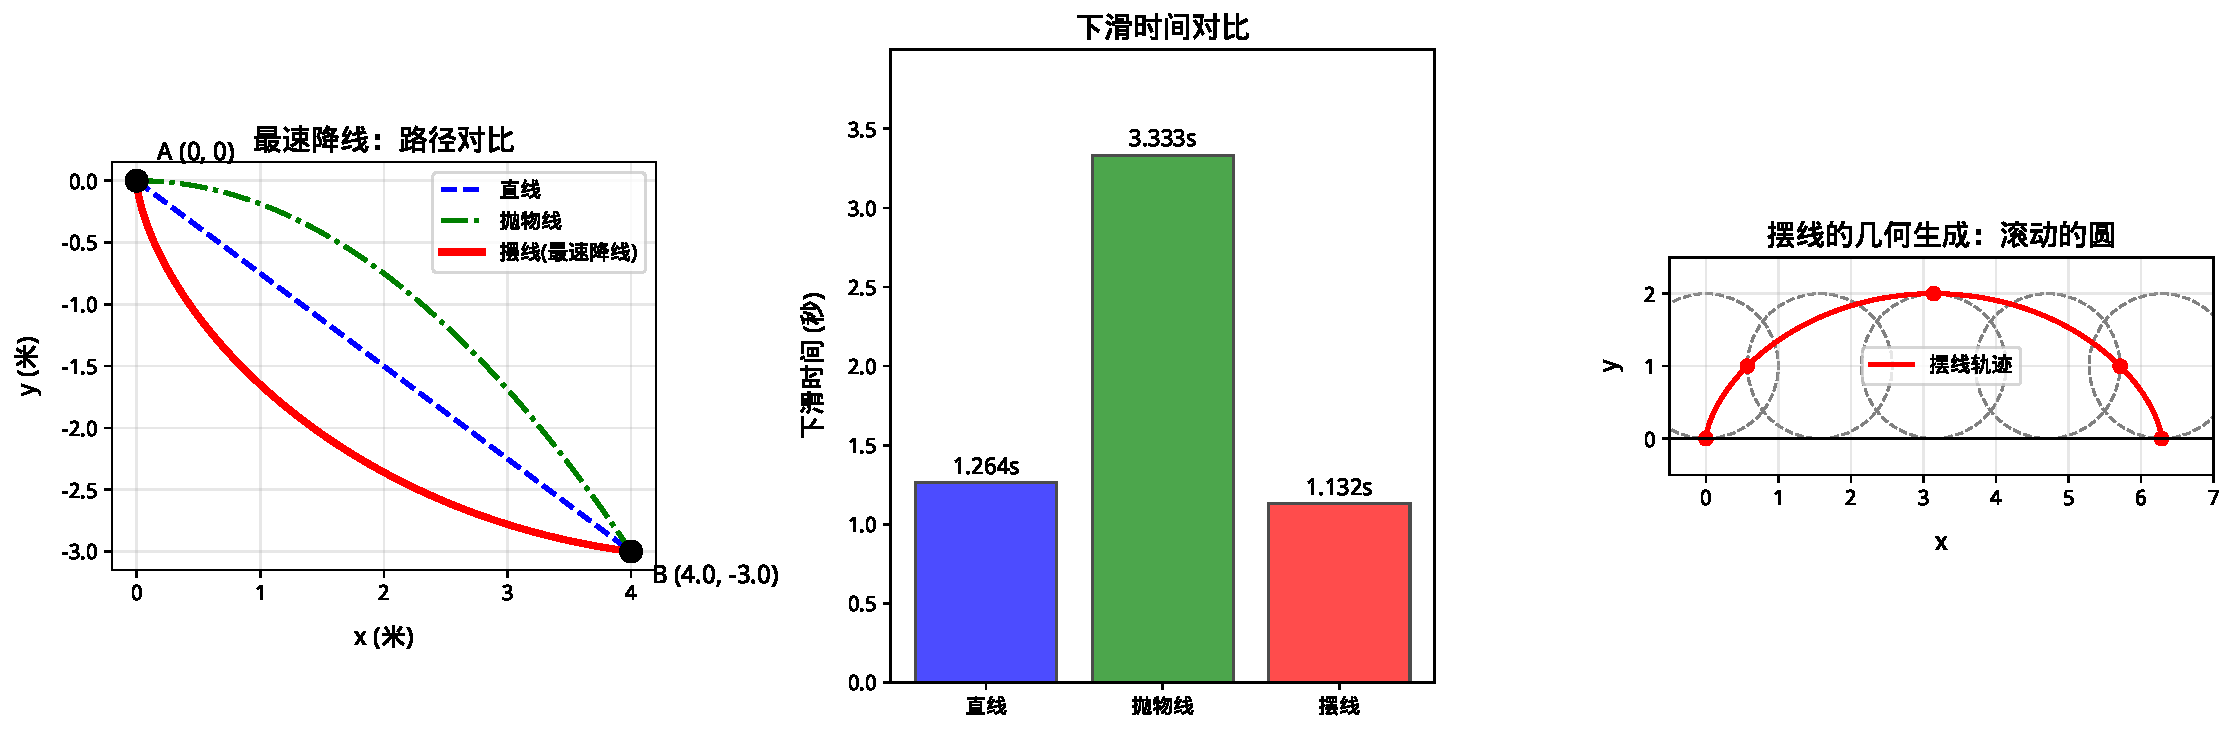
\includegraphics[width=0.95\textwidth]{figs_chap03/brachistochrone.pdf}
\caption{最速降线（Brachistochrone）问题演示。左图对比三种下滑路径：直线、抛物线和摆线；中图显示下滑时间对比——摆线确实是最快的，比直线快约10.5\%；右图展示摆线的几何生成原理：圆在直线上滚动，圆周上一点的轨迹即为摆线。}
\label{fig:chap03_brachistochrone}
\end{figure}

\begin{figure}[htbp]
\centering
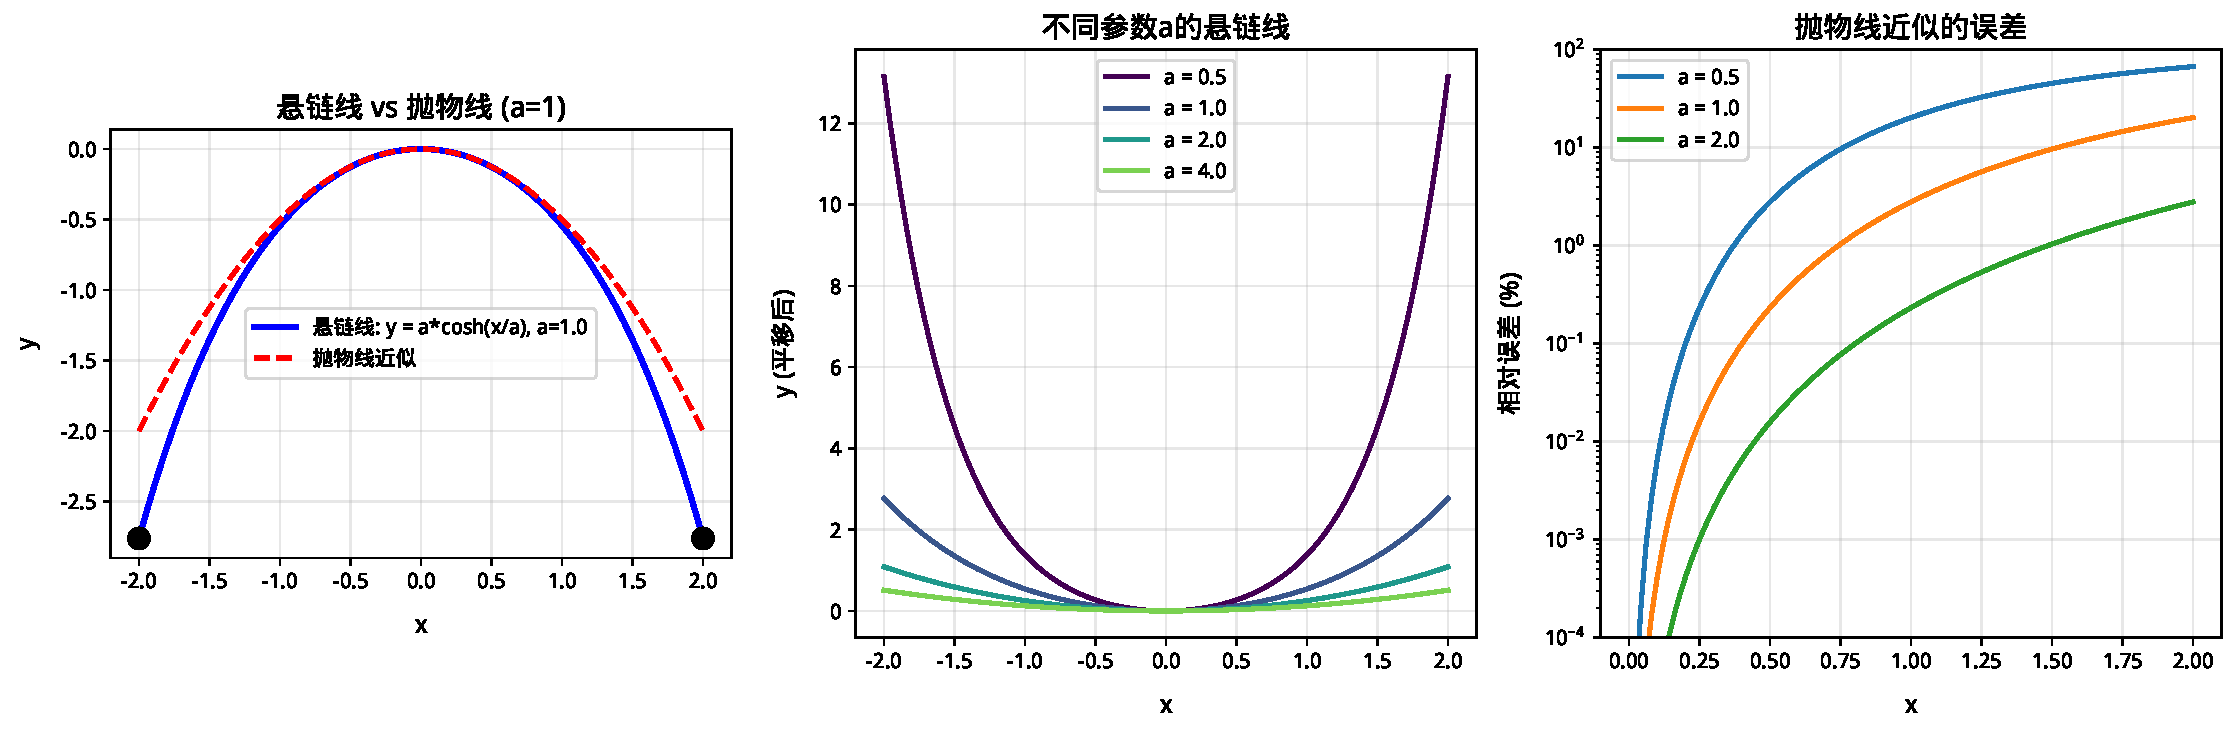
\includegraphics[width=0.95\textwidth]{figs_chap03/catenary.pdf}
\caption{悬链线问题演示。左图对比悬链线$y = a\cosh(x/a)$与抛物线近似（$a=1$时）——两者在中心区域接近，边缘处差异明显；中图展示不同$a$值对悬链线形状的影响——$a$越小，曲线越"尖"；右图显示抛物线近似的相对误差，说明在$|x|$较大时近似失效。}
\label{fig:chap03_catenary}
\end{figure}

% ------------------------------------------------------------------------------------
\section{本章小结}

\begin{enumerate}
    \item \textbf{泛函}：以函数为输入、数字为输出的映射。变分问题就是优化泛函。
    
    \item \textbf{核心观点}：变分法 = 无限维的拉格朗日乘子法。通过离散化，变分问题变成第1章的带约束优化问题。
    
    \item \textbf{Euler-Lagrange 方程}：泛函极值的必要条件
    \[
    \frac{\partial F}{\partial y} - \frac{d}{dx}\frac{\partial F}{\partial y'} = 0
    \]
    
    \item \textbf{守恒律}：
    \begin{itemize}
        \item $F$ 不含 $y$ $\Rightarrow$ $\frac{\partial F}{\partial y'}$ 守恒
        \item $F$ 不含 $x$ $\Rightarrow$ $F - y'\frac{\partial F}{\partial y'}$ 守恒（能量守恒）
    \end{itemize}
    
    \item \textbf{带约束的变分}：用拉格朗日乘子处理积分约束，和第1章方法完全一致。
    
    \item \textbf{经典例子}：
    \begin{itemize}
        \item 测地线（最短路径）→ 直线
        \item 悬链线（最小势能）→ $y = a\cosh(x/a)$
        \item 等周问题（最大面积）→ 圆
    \end{itemize}
\end{enumerate}

\begin{unification}[title=统一视角]
\begin{center}
\renewcommand{\arraystretch}{1.4}
\begin{tabular}{lll}
\toprule
& \textbf{有限维（第1章）} & \textbf{无限维（本章）} \\
\midrule
变量 & 向量 $\mathbf{x} \in \mathbb{R}^n$ & 函数 $y(x)$ \\
目标 & 函数 $f(\mathbf{x})$ & 泛函 $J[y]$ \\
约束 & $g(\mathbf{x}) = 0$ & $y_{k+1} - y_k = v_k \Delta x$ \\
乘子 & $\lambda$ & $\lambda_k = \frac{\partial F}{\partial v_k}$（动量） \\
必要条件 & $\nabla f + \lambda \nabla g = 0$ & E-L 方程 \\
影子价格 & $\frac{df^*}{dc}$ & $\frac{dJ^*}{dc}$（如等周问题中 $\lambda = r$） \\
\bottomrule
\end{tabular}
\end{center}

\textbf{核心洞察}：E-L 方程不是"新发明"，而是有限维乘子法的自然极限。

从下一章开始，我们将用这套语言重新理解自然界：先是"不确定性"（第4章的最大熵），再是牛顿力学与连续介质（第5、13章）——它们都可以看作变分问题！
\end{unification}

% ------------------------------------------------------------------------------------
\section{习题}

\paragraph{计算题}
\begin{enumerate}
    \item 用 E-L 方程求使 $\int_0^1 (y')^2 \, dx$ 最小的函数 $y(x)$，满足 $y(0) = 0$，$y(1) = 1$。
    
    \item 求使 $\int_0^{\pi} [(y')^2 - y^2] \, dx$ 取极值的函数，满足 $y(0) = 0$，$y(\pi) = 0$。
    
    \item 验证悬链线 $y = a\cosh(x/a)$ 满足势能泛函 $J[y] = \int y\sqrt{1+(y')^2} \, dx$ 的 E-L 方程。
    
    \item 用 Beltrami 恒等式（能量守恒）求解最速降线问题：
    \[
    J[y] = \int_0^{x_1} \frac{\sqrt{1+(y')^2}}{\sqrt{y}} \, dx
    \]
    其中 $y$ 向下为正。
\end{enumerate}

\paragraph{证明题}
\begin{enumerate}
    \setcounter{enumi}{4}
    \item 证明：若 $F$ 不显含 $y$，则 $\frac{\partial F}{\partial y'}$ 沿极值曲线为常数。
    
    \item 证明 Beltrami 恒等式：若 $F$ 不显含 $x$，则 $F - y'\frac{\partial F}{\partial y'} = C$。
    
    \item 用离散乘子法证明：对于离散变分问题，$\lambda_k = \frac{\partial F}{\partial v_k}$。（提示：这就是本章第四步）
    
    \item 证明等周问题的拉格朗日乘子 $\lambda$ 等于圆的半径 $r$。
\end{enumerate}

\paragraph{编程题}
\begin{enumerate}
    \setcounter{enumi}{8}
    \item 实现离散变分：
    \begin{enumerate}
        \item 把曲线长度泛函离散化为求和
        \item 用数值优化（如梯度下降）找最短曲线
        \item 验证结果收敛到直线
    \end{enumerate}
    
    \item 数值求解最速降线：
    \begin{enumerate}
        \item 离散化下滑时间泛函
        \item 用优化算法找最优曲线
        \item 与解析解（摆线）比较
        \item 统计时间节省百分比（相比直线）
    \end{enumerate}
    
    \item 实现离散拉格朗日乘子法：
    \begin{enumerate}
        \item 构造离散拉格朗日函数 $\mathcal{L}(\{y_k\}, \{v_k\}, \{\lambda_k\})$
        \item 解 KKT 条件（联立方程组）
        \item 验证 $\lambda_k$ 确实等于 $\frac{\partial F}{\partial v_k}$
    \end{enumerate}
\end{enumerate}

\paragraph{思考题}
\begin{enumerate}
    \setcounter{enumi}{11}
    \item 为什么物理学家喜欢用变分原理（最小作用量）而不是直接用牛顿定律？
    
    \item 本章用"离散化 → 乘子法 → 取极限"推导 E-L 方程。这个思路能否推广到偏微分方程（如波动方程、热传导方程）？
    
    \item 神经网络可以看作是泛函的离散化吗？从这个角度理解物理信息神经网络（PINN）。
    
    \item 机器学习中的"正则化"（如 $L_2$ 正则化）和变分问题中的"光滑性泛函"有什么联系？
\end{enumerate}